\documentclass[dvipdfmx,9pt]{beamer}
\usepackage{bxdpx-beamer}
\usepackage{minijs}
\renewcommand{\kanjifamilydefault}{\gtdefault}
\usetheme{metropolis}
\setbeamercolor{background canvas}{bg = yellow!5!white}
\usefonttheme{professionalfonts}
\usepackage{amsmath, amsfonts,bm,graphicx,here,tikz,mathtools,physics}
\graphicspath{{../images/}}
\usepackage{hyperref}
\usepackage{pxjahyper}
\hypersetup{
    setpagesize=false,
    bookmarksnumbered=true,
    bookmarksopen=true,
    colorlinks=true,
    linkcolor=green!50!blue!60!white!65!black,
    citecolor=green!50!blue!80!black,
    urlcolor=green!60!yellow!75!red!85!blue
}
\newcommand{\del}{\partial}
\newcommand{\dblpi}{(2\pi)}
\newcommand{\kb}{k_\mathrm{B}}
\numberwithin{equation}{section}
\begin{document}
\title{ファインマン統計力学 7章}
\subtitle{スピン波}
\author{政岡凜太郎}
\frame{\titlepage}

\section{Bethe仮設}
\begin{frame}{2個のスピン波 (厳密な取り扱い)}
    ここではBetheによる1次元Heisenberg模型の厳密な取り扱いを,スピン波が2個の場合に行う.まず真空を
    \begin{align}
        \ket{0} \equiv \ket{\uparrow \cdots \uparrow}
    \end{align}
    と定義する.強磁性の場合は真空が基底状態となる.また$n$粒子状態を
    \begin{align}
        \ket{x_1, x_2, \ldots, x_n} = \sigma_{x_1}^- \sigma_{x_2}^- \cdots \sigma_{x_n}^-\ket{0}
    \end{align}
    とおく.ただし$x_1 < x_2 < \cdots < x_n$とする.
    2粒子状態の固有状態として,以下の形のものを仮設する.
    \begin{gather}
        \ket{\psi} = \sum_{1 \le x_1 < x_2 \le N} \psi(x_1, x_2)\ket{x_1, x_2},
        \\[5pt]
        \psi(x_1, x_2) = A_{12}e^{i(k_1 x_1 + k_2 x_2)} + A_{21}e^{i(k_2 x_1 + k_1 x_2)}.
        \label{2 spin waves: Bethe ansatz wave function}
    \end{gather}
    Bethe仮設法においては,まず解の形を仮定して,あとでそれが厳密解であることを示す.
\end{frame}

\begin{frame}{}
    \begin{align}
        \psi(x_2, x_1+N) = \psi(x_1, x_2)
    \end{align}
    \begin{align}
        e^{ik_2N}A_{12} = A_{21},
        \quad
        e^{ik_1N}A_{21} = A_{12}
    \end{align}
    \begin{align}
        H \ket{\psi} = 4\epsilon J\ket{\psi}
    \end{align}
    \begin{align}
        H = -J\sum_i \bm{\sigma}_i \cdot \bm{\sigma}_{i+1} + NJ = -2J\sum_i (\Pi^{i,i+1}-1)
        \label{2 spin waves: Sch-eq}
    \end{align}
\end{frame}

\begin{frame}{}
    (\ref{2 spin waves: Sch-eq})を$\ket{x_1, x_2}$を基底として展開したときの成分を考える.$x_2 - x_1 > 1$のとき,
    \begin{align}
        4\epsilon J\psi(x_1, x_2) = &
        -2J\Big[
            \psi(x_1-1, x_2) + \psi(x_1+1, x_2) \nonumber
        \\ & \qquad\quad
        + \psi(x_1, x_2-1) + \psi(x_1, x_2+1) - 4\psi(x_1, x_2)\Big].
        \label{2 spin waves: Sch-eq about psi}
    \end{align}
    \begin{figure}[H]
        \centering
        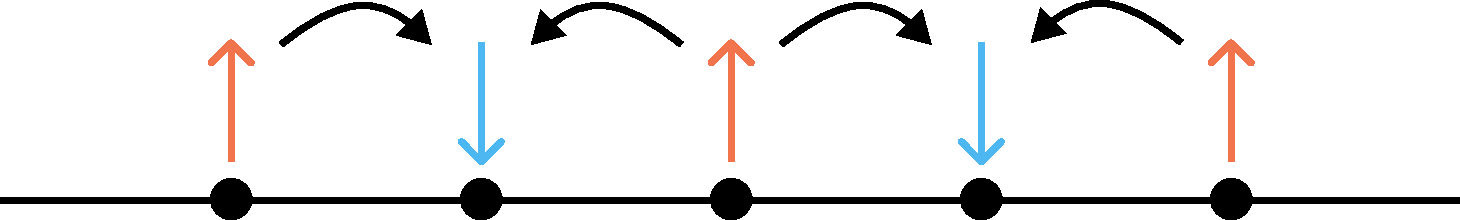
\includegraphics[scale = 0.3]{i1.pdf}
    \end{figure}
    さらに,$A_{12}\exp(i(k_1 x_1 + k_2 x_2))$に掛かる係数だけを取り出すと,
    \begin{align}
        \epsilon
        &\nonumber
        = -\frac{1}{2}(e^{-ik_1} + e^{ik_1} + e^{-ik_2} + e^{ik_2} - 4)
        \\ &
        = 2-\cos{k_1}-\cos{k_2}
    \end{align}

\end{frame}

\begin{frame}{}
    次に$x_2 - x_1 = 1$のとき,
    \begin{align}
        4\epsilon J\psi(x_1, x_2) = -2J \qty\Big[\psi(x_1-1,x_2) + \psi(x_1,x_2+1) - 2\psi(x_1,x_2)].
    \end{align}
    \begin{figure}[H]
        \centering
        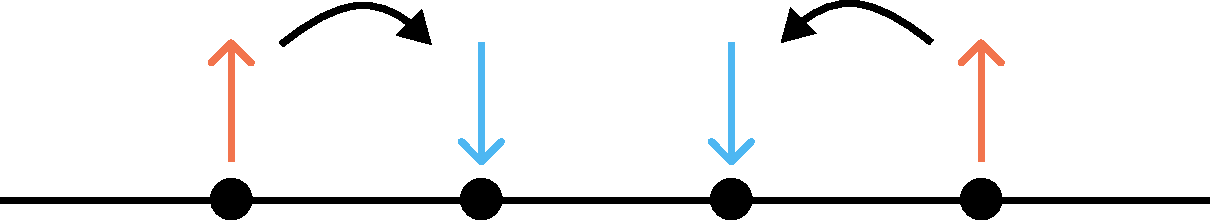
\includegraphics[scale = 0.3]{i2.pdf}
    \end{figure}
    これが(\ref{2 spin waves: Sch-eq about psi})と整合するように,境界条件
    \begin{align}
        2\psi(x, x+1) = \psi(x, x) + \psi(x+1,x+1)
    \end{align}
    を課す.($\psi(x,x)$はまだ定義されていなかった).
    したがって,
    \begin{gather}
        2(A_{12}e^{ik_2} + A_{21}e^{ik_1})
        = (A_{12}+A_{21})\qty(1+e^{i(k_1+k_2)})
        \label{2 spin waves: connection condition}
    \end{gather}
    となる.
\end{frame}

\begin{frame}{}
    (\ref{2 spin waves: connection condition})を整理すると,
    \begin{align}
        \frac{A_{12}}{A_{21}} &
        = -\frac{1+e^{i(k_1+k_2)}-2e^{ik_1}}{1+e^{i(k_1+k_2)}-2e^{ik_2}}
    \end{align}
    となる.ここで,ラピディティ$\lambda_j$を
    \begin{align}
        e^{ik_j} = \frac{\lambda_j + i}{\lambda_j - i}
    \end{align}
    で定義すれば,
    \begin{align}
        \frac{A_{12}}{A_{21}} &\nonumber
        = -\frac{(\lambda_1-i)(\lambda_2-i) + (\lambda_1+i)(\lambda_2+i) - 2(\lambda_1+i)(\lambda_2-i)}
        {(\lambda_1-i)(\lambda_2-i) + (\lambda_1+i)(\lambda_2+i) - 2(\lambda_1-i)(\lambda_2+i)}
        \\ &
        = \frac{2i\lambda_1 - 2i\lambda_2 - 4}
        {2i\lambda_1 - 2i\lambda_2 + 4}
        = \frac{\lambda_1-\lambda_2+2i}
        {\lambda_1-\lambda_2-2i}
    \end{align}
    となる.ここから
    \begin{align}
        \qty(\frac{\lambda_1+i}{\lambda_1-i})^N = \frac{\lambda_1-\lambda_2+2i}
        {\lambda_1-\lambda_2-2i}
    \end{align}
    を得る.これと添字$1,2$を入れ替えた式をまとめてBethe仮設方程式という.
\end{frame}

% \begin{frame}
%     (\ref{2 spin waves: connection condition})を整理すると,
%     \begin{align}
%         \frac{A_{12}}{A_{21}} &
%         = -\frac{1+e^{i(k_1+k_2)}-2e^{ik_2}}{1+e^{i(k_1+k_2)}-2e^{ik_1}}
%         \\[5pt] &
%         = -\frac{\cos{\frac{k_1+k_2}{2}}-e^{i(k_1-k_2)/2}}{\cos{\frac{k_2+k_1}{2}}-e^{i(k_2-k_1)/2}}.
%     \end{align}
%     $k_1,k_2$が実数ならば,分母と分子は複素共役の関係にあり,
%     \begin{align}
%         \frac{A_{12}}{A_{21}} = \frac{z}{z^*}, 
%         \quad z = i \cos \frac{k_1+k_2}{2} - ie^{i(k_1-k_2)/2}
%     \end{align}
%     となる.$A_{12}/A_{21} = e^{i\varphi}$とおけば,
%     \begin{align}
%         \cot \frac{\varphi}{2} = \frac{\Re z}{\Im z} &= \frac{\sin \frac{k_1-k_2}{2}}{\cos \frac{k_1+k_2}{2}-\cos \frac{k_1-k_2}{2}}
%         \\ &
%         = \frac{\sin \frac{k_1}{2}\cos \frac{k_2}{2} - \cos \frac{k_1}{2} \sin \frac{k_2}{2}}{-\sin \frac{k_1}{2} \sin \frac{k_2}{2}}
%         \\ &
%         = \cot \frac{k_1}{2} - \cot \frac{k_2}{2}
%     \end{align}
% \end{frame}

\begin{frame}{ストリング解}
    $\lambda_1, \lambda_2$は実数とは限らない.ここでは,
    \begin{align}
        \lambda_1 = \lambda + i + i\epsilon,
        \\
        \lambda_2 = \lambda - i - i\epsilon.
    \end{align}
    という解を考える.
    \begin{align}
        \qty(\frac{\lambda + 2i}{\lambda})^N = \frac{4i}{2i\epsilon}
    \end{align}
    \begin{align}
        e^{ik_1} = \frac{\lambda + 2i}{\lambda},
        \quad
        e^{ik_2} = \frac{\lambda}{\lambda - 2i} = e^{ik_1^*}
    \end{align}
    \begin{align}
        k_1 = u+iv,\quad k_2 = u-iv
    \end{align}
    \begin{align}
        \Re e^{ik_1} = e^{-v}\cos u = 1
    \end{align}
\end{frame}

\begin{frame}{}
    \begin{align}
        e^{i(k_1+k_2)N} = e^{2iuN} = 1
    \end{align}
    \begin{align}
        \psi(x_1, x_2) = A_{12}e^{iu(x_1+x_2)}e^{v(x_2-x_1)} + A_{21}e^{iu(x_1+x_2)}e^{-v(x_2-x_1)}
    \end{align}
    \begin{align}
        \qty|\frac{A_{12}}{A_{21}}| = |e^{ik_1 N}| = e^{-vN} \ll 1
    \end{align}
\end{frame}
\begin{frame}
    \begin{align}
        \epsilon &= 2 - \cos(u+iv)-\cos(u-iv) 
        \\ &
        = 2(1-\cos u \cosh v)
        \\ &
        = 2\qty(1- \cos u \cdot \frac{1}{2}\qty(\cos u + \frac{1}{\cos u}))
        \\ &
        = \sin^2 u
        = \frac{1}{2}(1-\cos (k_1+k_2))
    \end{align}
    \begin{align}
        \frac{E}{4J} = 2(1- \cos K) = K^2 - \frac{K^4}{12} + \cdots
    \end{align}
    \begin{align}
        \frac{E}{4J} = \frac{1}{2}(1-\cos 2K) = K^2 - \frac{K^4}{3} + \cdots
    \end{align}
    したがってマグノン同士の結合エネルギーは$JK^4$である.
\end{frame}

\begin{frame}{$M$個のスピン波}
    $M$個のスピン波を表す状態を$\ket*{\psi^{(M)}}$と書き,
    \begin{align}
        \ket*{\psi^{(M)}} = \sum_{1\le x_1 < \cdots < x_M \le N}  \psi(x_1,\ldots,x_M) \ket{x_1,\ldots,x_M}
    \end{align}
    と展開する.Bethe仮設波動関数を
    \begin{align}
        \psi(x_1,\ldots,x_M) = \sum_{P \in S_M} A_P \exp(i \sum_{j=1}^M k_{Pj} x_j)
    \end{align}
    と定義する.
\end{frame}
\begin{frame}
    周期的境界条件は
    \begin{align}
        \psi(x_2,\ldots,x_M,x_1+N) = \psi(x_1,x_2,\ldots,x_M)
    \end{align}
    となる.左辺を計算すると,
    \begin{align}
        \psi(x_2,\ldots,x_M,x_1+N)
        &
        = \sum_{P \in S_M} e^{k_{PM}N} A_P \exp(i \sum_j k_{Pj}x_{j+1})
        \\ &
        = \sum_{P \in S_M} e^{k_{P1}N} A_{PR} \exp(i \sum_j k_{Pj}x_j).
    \end{align}
    ただし$R$は巡回置換$j \mapsto j+1$を表す.したがって,
    \begin{align}
        e^{i k_{P1}N}A_{PR} = A_P,
        \quad
        \frac{A_{PR}}{A_P} = e^{i k_{P1}N}
    \end{align}
\end{frame}

\begin{frame}
    次に固有値方程式にBethe波動関数を代入する.まず,
    \begin{align}
        |x_1-x_2|>1,~ |x_2-x_3|>1,\ldots,~ |x_{M-1}-x_M|>1
    \end{align}
    のとき,
    \begin{align}
        E\psi(x_1,\ldots,x_M) = 
        \sum_{j=1}^M \sum_{\xi=\pm 1} (\psi(\ldots,x_j+\xi,\ldots)-\psi(\ldots,x_j,\ldots))
        \label{Bethe Ansatz: eigenvalue condition}
    \end{align}
    となる.次に$x_{j+1}=x_j+1$の場合にこの式を適用すると,$\psi(\ldots,x_j,x_j,\ldots)$という項と$\psi(\ldots,x_j+1,x_j+1,\ldots)$という項が出てくる.
    そこで,境界条件
    \begin{align}
        & \nonumber
        2\psi(\ldots,x_j,x_j+1,\ldots)
        \\ &
        = \psi(\ldots,x_j,x_j,\ldots)+ \psi(\ldots,x_j+1,x_j+1,\ldots)
        \label{Bethe Ansatz: M particle boundary condition}
    \end{align}
    を課す.すると余計な項による寄与が消えてくれて,(\ref{Bethe Ansatz: eigenvalue condition})が任意の場合に成り立つ.
\end{frame}

\begin{frame}
    (\ref{Bethe Ansatz: M particle boundary condition})を係数$A(P)$で表そう.まず$M=3$の場合を考えてみる.
    \begin{align}
        2\psi(x_1,x_2,x_2+1) = \psi(x_1,x_2,x_2+1) + \psi(x,x_2+1,x_2+1)
        \label{Bethe Ansatz: 3 particle boundary condition}
    \end{align}
    という式に,
    \begin{align}
        \psi(x_1,x_2,x_3) &\nonumber
        = A_{123}e^{i(k_1x_1+k_2x_2+k_3x_3)}
        \\ & \quad
        + A_{132}e^{i(k_1x_1 + k_3x_2 + k_2x_3)} + \cdots
        \label{Bethe Ansatz: 3 wave function}
    \end{align}
    を代入する.
    (\ref{Bethe Ansatz: 3 particle boundary condition})の中で$x_1$依存性が$e^{ik_1 x_1}$という形になる項だけを取り出せば,(\ref{Bethe Ansatz: 3 wave function})の最初の2項を考えるだけでよく,
    \begin{align}
        2\qty(A_{123}e^{ik_3} + A_{132}e^{ik_2}) = (A_{123} + A_{132})\qty(1 + e^{i(k_3+k_2)})
    \end{align}
    を得る.同様にして,
    \begin{align}
        2\qty(A_{231}e^{ik_1}+A_{213}e^{ik_3}) = (A_{231}+A_{213})\qty(1+e^{i(k_1+k_3)})
        \\
        2\qty(A_{312}e^{ik_2}+A_{321}e^{ik_1}) = (A_{312}+A_{321})\qty(1+e^{i(k_2+k_1)})
    \end{align}
    を得る.
\end{frame}

\begin{frame}
    $M$粒子の場合も同様に考えられる.$\pi_j$を$j$と$j+1$を入れ替える置換とすれば,
    \begin{align}
        &\nonumber
        2\qty(A_P e^{ik_{P(j+1)}}+A_{P\pi_j}e^{ik_{Pj}})
        \\ &
        = (A_P+A_{P\pi_j})\qty(1+\exp{i(k_{P(j+1)}+k_{Pj})})
    \end{align}
    \begin{align}
        \frac{A_{P\pi_j}}{A_P} = -\frac{1+\exp{i(k_{P(j+1)}+k_{Pj})}-2\exp(k_{Pj})}{1+\exp{i(k_{Pj}+k_{P(j+1)})}-2\exp(ik_{P(j+1)})}
    \end{align}
    となる.2粒子の場合と同様にラピディティを
    \begin{align}
        e^{ik_j} = \frac{\lambda_j + i}{\lambda_j - i}
    \end{align}
    で定義すれば,
    \begin{align}
        \frac{A_{P\pi_j}}{A_P} = \frac{\lambda_{Pj}-\lambda_{P(j+1)}+2i}{\lambda_{Pj}-\lambda_{P(j+1)}-2i}
    \end{align}
\end{frame}
\begin{frame}
    \begin{align}
        R = \pi_1 \pi_2 \cdots \pi_{M-1}
    \end{align}
    $R_j = \pi_1 \pi_2 \cdots \pi_{j-2}\pi_{j-1}$とすると,$R_{M} = R,~ R_1 = e$であり,
    \begin{align}
        \frac{A_{PR}}{A_P}
        = \frac{A_{PR_M}}{A_{R_{M-1}}}
        \frac{A_{PR_{M-1}}}{A_{PR_{M-2}}} \cdots \frac{A_{PR_3}}{A_{PR_2}} \frac{A_{PR_2}}{A_{PR_1}}
    \end{align}
    と分解できる.ここで,$R_j j = 1,~R_j(j+1) = j+1$であるから,
    \begin{align}
        \frac{A_{PR_{j+1}}}{A_{PR_j}} = \frac{A_{PR_j \pi_j}}{A_{PR_j}} = \frac{\lambda_{P1}-\lambda_{P(j+1)}+2i}{\lambda_{P1}-\lambda_{P(j+1)}-2i}
    \end{align}
    である.これを$j+1 = 2,3,\ldots,M$の場合で掛け合わせて,
    \begin{align}
        \frac{A_{PR}}{A_P} = \prod_{l \ne P1}\frac{\lambda_{P1}-\lambda_-+2i}{\lambda_{P1}-\lambda_--2i}
    \end{align}
    を得る.
\end{frame}

\begin{frame}
    \begin{align}
        \qty(\frac{\lambda_j + i}{\lambda_j - i})^N = \prod_{l \ne j}\frac{\lambda_{j}-\lambda_-+2i}{\lambda_{j}-\lambda_--2i},
        \quad
        (j = 1,2,\ldots,M)
    \end{align}
\end{frame}

\begin{frame}{反強磁性Heisenberg模型の基底状態}
    
\end{frame}

\begin{frame}{スピノン}
    
\end{frame}
\end{document}